% Hat functions on a uniform mesh and a P1 interpolant. Generated by a short script.
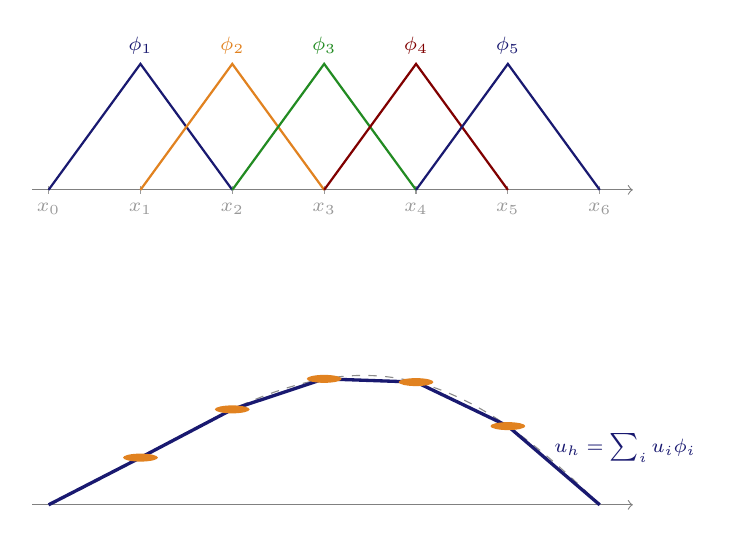
\begin{tikzpicture}[xscale=7,yscale=1.6]
\draw[->,black!50] (-0.03,0) -- (1.06,0);
\draw[black!40] (0.0000,0.03) -- (0.0000,-0.03) node[below,font=\scriptsize] {$x_0$};
\draw[black!40] (0.1667,0.03) -- (0.1667,-0.03) node[below,font=\scriptsize] {$x_1$};
\draw[black!40] (0.3333,0.03) -- (0.3333,-0.03) node[below,font=\scriptsize] {$x_2$};
\draw[black!40] (0.5000,0.03) -- (0.5000,-0.03) node[below,font=\scriptsize] {$x_3$};
\draw[black!40] (0.6667,0.03) -- (0.6667,-0.03) node[below,font=\scriptsize] {$x_4$};
\draw[black!40] (0.8333,0.03) -- (0.8333,-0.03) node[below,font=\scriptsize] {$x_5$};
\draw[black!40] (1.0000,0.03) -- (1.0000,-0.03) node[below,font=\scriptsize] {$x_6$};
\draw[MidnightBlue,thick] (0.0000,0) -- (0.1667,1) -- (0.3333,0);
\node[MidnightBlue,above,font=\scriptsize] at (0.1667,1) {$\phi_1$};
\draw[BurntOrange!90!black,thick] (0.1667,0) -- (0.3333,1) -- (0.5000,0);
\node[BurntOrange!90!black,above,font=\scriptsize] at (0.3333,1) {$\phi_2$};
\draw[ForestGreen,thick] (0.3333,0) -- (0.5000,1) -- (0.6667,0);
\node[ForestGreen,above,font=\scriptsize] at (0.5000,1) {$\phi_3$};
\draw[Maroon,thick] (0.5000,0) -- (0.6667,1) -- (0.8333,0);
\node[Maroon,above,font=\scriptsize] at (0.6667,1) {$\phi_4$};
\draw[MidnightBlue,thick] (0.6667,0) -- (0.8333,1) -- (1.0000,0);
\node[MidnightBlue,above,font=\scriptsize] at (0.8333,1) {$\phi_5$};
\begin{scope}[yshift=-2.5cm]
\draw[->,black!50] (-0.03,0) -- (1.06,0);
\draw[black!45,dashed] (0.0000,0.0000) -- (0.0083,0.0165) -- (0.0167,0.0334) -- (0.0250,0.0505) -- (0.0333,0.0679) -- (0.0417,0.0857) -- (0.0500,0.1036) -- (0.0583,0.1219) -- (0.0667,0.1403) -- (0.0750,0.1590) -- (0.0833,0.1779) -- (0.0917,0.1970) -- (0.1000,0.2163) -- (0.1083,0.2358) -- (0.1167,0.2553) -- (0.1250,0.2751) -- (0.1333,0.2949) -- (0.1417,0.3148) -- (0.1500,0.3348) -- (0.1583,0.3549) -- (0.1667,0.3750) -- (0.1750,0.3951) -- (0.1833,0.4153) -- (0.1917,0.4354) -- (0.2000,0.4555) -- (0.2083,0.4756) -- (0.2167,0.4956) -- (0.2250,0.5155) -- (0.2333,0.5353) -- (0.2417,0.5550) -- (0.2500,0.5745) -- (0.2583,0.5939) -- (0.2667,0.6131) -- (0.2750,0.6321) -- (0.2833,0.6509) -- (0.2917,0.6694) -- (0.3000,0.6877) -- (0.3083,0.7057) -- (0.3167,0.7234) -- (0.3250,0.7407) -- (0.3333,0.7578) -- (0.3417,0.7745) -- (0.3500,0.7908) -- (0.3583,0.8067) -- (0.3667,0.8222) -- (0.3750,0.8373) -- (0.3833,0.8519) -- (0.3917,0.8661) -- (0.4000,0.8797) -- (0.4083,0.8929) -- (0.4167,0.9056) -- (0.4250,0.9177) -- (0.4333,0.9292) -- (0.4417,0.9402) -- (0.4500,0.9507) -- (0.4583,0.9605) -- (0.4667,0.9697) -- (0.4750,0.9782) -- (0.4833,0.9861) -- (0.4917,0.9934) -- (0.5000,1.0000) -- (0.5083,1.0059) -- (0.5167,1.0111) -- (0.5250,1.0156) -- (0.5333,1.0194) -- (0.5417,1.0224) -- (0.5500,1.0247) -- (0.5583,1.0263) -- (0.5667,1.0271) -- (0.5750,1.0271) -- (0.5833,1.0263) -- (0.5917,1.0247) -- (0.6000,1.0224) -- (0.6083,1.0192) -- (0.6167,1.0153) -- (0.6250,1.0105) -- (0.6333,1.0049) -- (0.6417,0.9985) -- (0.6500,0.9912) -- (0.6583,0.9832) -- (0.6667,0.9743) -- (0.6750,0.9645) -- (0.6833,0.9540) -- (0.6917,0.9426) -- (0.7000,0.9304) -- (0.7083,0.9173) -- (0.7167,0.9034) -- (0.7250,0.8887) -- (0.7333,0.8732) -- (0.7417,0.8568) -- (0.7500,0.8397) -- (0.7583,0.8217) -- (0.7667,0.8030) -- (0.7750,0.7834) -- (0.7833,0.7631) -- (0.7917,0.7419) -- (0.8000,0.7200) -- (0.8083,0.6974) -- (0.8167,0.6740) -- (0.8250,0.6499) -- (0.8333,0.6250) -- (0.8417,0.5994) -- (0.8500,0.5732) -- (0.8583,0.5462) -- (0.8667,0.5186) -- (0.8750,0.4903) -- (0.8833,0.4614) -- (0.8917,0.4319) -- (0.9000,0.4017) -- (0.9083,0.3710) -- (0.9167,0.3397) -- (0.9250,0.3079) -- (0.9333,0.2755) -- (0.9417,0.2426) -- (0.9500,0.2092) -- (0.9583,0.1754) -- (0.9667,0.1411) -- (0.9750,0.1064) -- (0.9833,0.0713) -- (0.9917,0.0358) -- (1.0000,0.0000);
\draw[MidnightBlue,very thick] (0.0000,0.0000) -- (0.1667,0.3750) -- (0.3333,0.7578) -- (0.5000,1.0000) -- (0.6667,0.9743) -- (0.8333,0.6250) -- (1.0000,0.0000);
\fill[BurntOrange!90!black] (0.1667,0.3750) circle (0.9pt);
\fill[BurntOrange!90!black] (0.3333,0.7578) circle (0.9pt);
\fill[BurntOrange!90!black] (0.5000,1.0000) circle (0.9pt);
\fill[BurntOrange!90!black] (0.6667,0.9743) circle (0.9pt);
\fill[BurntOrange!90!black] (0.8333,0.6250) circle (0.9pt);
\node[MidnightBlue,font=\scriptsize,right] at (0.9,0.45) {$u_h=\sum_iu_i\phi_i$};
\end{scope}
\end{tikzpicture}
